% ------------------------------------------------------------------------------
% TYPO3 CMS 7.3 - What's New (English Version)
%
% @author	Michael Schams <schams.net>
% @license	Creative Commons BY-NC-SA 3.0
% @link		http://typo3.org/download/release-notes/whats-new/
% @language	English
% ------------------------------------------------------------------------------
% LTXE-CHAPTER-UID:		cc6b358d-f0ed36d3-f7a72fa2-af63ccfc
% LTXE-CHAPTER-NAME:	Backend User Interface
% ------------------------------------------------------------------------------

\section{Backend Gebruikersinterface}

% ------------------------------------------------------------------------------
% LTXE-SLIDE-START
% LTXE-SLIDE-UID:		10b9c886-883896f7-fd5b31d9-23523ecb
% LTXE-SLIDE-ORIGIN:	111332b8-ac46a07a-319ed582-f873bc02 English
% LTXE-SLIDE-ORIGIN:	b4dc1576-57b4854f-26a32d85-11f7c52b German
% LTXE-SLIDE-TITLE:		Feature #66173: Allow page title edit by doubleclick
% LTXE-SLIDE-REFERENCE:	Feature-66173-AllowPageTitleEditByDoubleclick.rst
% ------------------------------------------------------------------------------
\begin{frame}[fragile]
	\frametitle{Backend Gebruikersinterface}
	\framesubtitle{Paginatitel in Pagina- en Lijstmodule}

	De paginatitel kan in de modules "Pagina" en "Lijst" gewijzigd worden door te dubbelklikken op de kop of
	of via het pictogram "Bewerken".

	\begin{figure}
		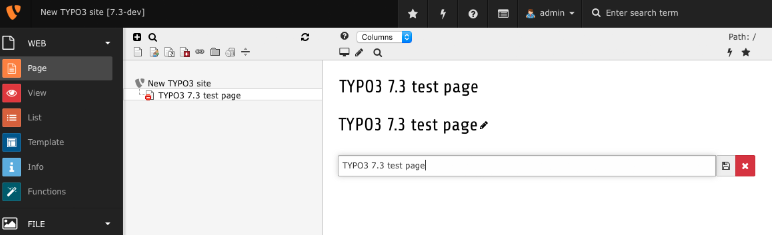
\includegraphics[width=0.9\linewidth]{BackendUserInterface/66173.png}
	\end{figure}

\end{frame}

% ------------------------------------------------------------------------------
% LTXE-SLIDE-START
% LTXE-SLIDE-UID:		fa50cffb-5db71fb9-e16283d7-9db71aaf
% LTXE-SLIDE-ORIGIN:	c17b263e-12512d4b-13d5389f-df1ec14e English
% LTXE-SLIDE-ORIGIN:	168b1424-1ebb2552-ed5bac3e-8a9ac737 German
% LTXE-SLIDE-TITLE:		Feature #67071: Processed files cleanup tool added in Install Tool
% LTXE-SLIDE-REFERENCE:	Feature-67071-ProcessedFilesCleanupToolAddedInInstallTool.rst
% ------------------------------------------------------------------------------
\begin{frame}[fragile]
	\frametitle{Backend Gebruikersinterface}
	\framesubtitle{Install Tool: bewerkte bestanden verwijderen}

	In het deel "Clean up" van de Install Tool zit een nieuwe functie om bewerkte bestanden
	(bijv. verkleinde voorbeelden van afbeeldingen) uit FAL te verwijderen.\newline
	Dit is handig als instellingen voor afbeeldingen zijn gewijzigd of na een update van
	GraphicsMagick/ImageMagick om te forceren dat alle afbeeldingen opnieuw aangemaakt
	worden.

	\begin{figure}
		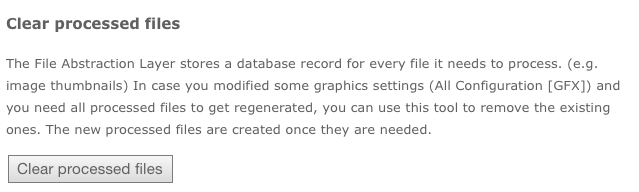
\includegraphics[width=0.6\linewidth]{BackendUserInterface/67071.png}
	\end{figure}

\end{frame}

% ------------------------------------------------------------------------------
% LTXE-SLIDE-START
% LTXE-SLIDE-UID:		39e8d6c9-bd63b353-11dde3f9-3e60d9ff
% LTXE-SLIDE-ORIGIN:	4662a0fc-e8a91f22-2f75e0bc-800e9b63 English
% LTXE-SLIDE-ORIGIN:	daa83c1e-08d2716b-de74cbda-42361551 German
% LTXE-SLIDE-TITLE:		Feature #67319: Add field "copyright" to EXT:filemetadata
% LTXE-SLIDE-REFERENCE:	Feature-67319-AddFieldCopyrightToEXTfilemetadata.rst
% ------------------------------------------------------------------------------
\begin{frame}[fragile]
	\frametitle{Backend Gebruikersinterface}
	\framesubtitle{Nieuw veld in FAL Metadata}

	Het veld "\textbf{Auteursrechten}" is toegevoegd aan de metadata van een FAL-record
	(systeemextensie: \texttt{filemetadata}).

	\begin{figure}
		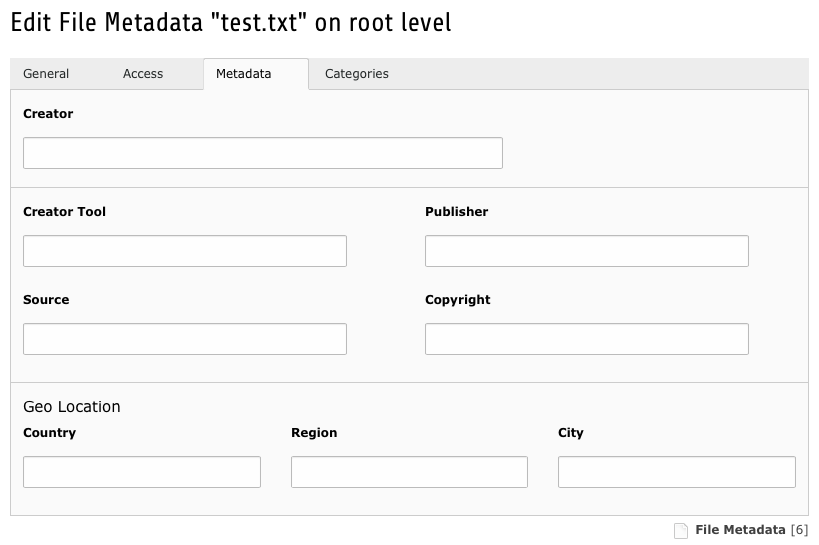
\includegraphics[width=0.6\linewidth]{BackendUserInterface/67319.png}
	\end{figure}

\end{frame}

% ------------------------------------------------------------------------------
